
%%%%%%%%%%%%%%%%%%%%%%%%%%%%%%%%%%%%%%%%%%%%%%%%%%
% Basic setup. Most papers should leave these options alone.
\documentclass[fleqn,usenatbib]{mnras}

\usepackage[T1]{fontenc}
\DeclareRobustCommand{\VAN}[3]{#2}
\let\VANthebibliography\thebibliography
\def\thebibliography{\DeclareRobustCommand{\VAN}[3]{##3}\VANthebibliography}

%%%%% AUTHORS - PLACE YOUR OWN PACKAGES HERE %%%%%
\usepackage{graphicx}	% Including figure files
\usepackage{amsmath}	% Advanced maths commands
\usepackage{amssymb}	% Extra maths symbols
\usepackage{xspace} 
\usepackage{xcolor}
\usepackage{upgreek}
\usepackage{CJK}
\usepackage{fontawesome}
\usepackage{gensymb}
\usepackage{multirow}
\usepackage{mathtools}
\usepackage{newtxtext,newtxmath}

%%%%% AUTHORS - PLACE YOUR OWN COMMANDS HERE %%%%%
\newcommand{\ToDo}[1]{\textbf{\textcolor{blue}{ToDo: #1}}}
\newcommand{\SB}[1]{{\textcolor{orange}{SB: #1}}}
\newcommand{\LM}[1]{{\textcolor{purple}{LM: #1}}}
\newcommand{\TB}[1]{{\textcolor{green}{TB: #1}}}
\newcommand{\Gaia}{\textit{Gaia}\xspace} % \Gaia

%%%%%%%%%%%%%%%%%%%%%%%%%%%%%%%%%%%%%%%%%%%%%%%%%%
%%%%%%%%%%%%%%%%%%% TITLE PAGE %%%%%%%%%%%%%%%%%%%

% Title of the paper, and the short title which is used in the headers.
% Keep the title short and informative.
\title[NIHAO vs. Milky Way: Radial metallicity gradients]{More than just a line? Shining light on the radial metallicity gradient with a NIHAO Milky-Way analogue simulation}

% The list of authors, and the short list which is used in the headers.
% If you need two or more lines of authors, add an extra line using \newauthor
\author[S. Buder and T. Buck]{
S. Buder,$^{1,2}$\thanks{E-mail: sven.buder@anu.edu.au} and
T. Buck,$^{3,4}$
\\
% List of institutions
$^{1}$Research School of Astronomy \& Astrophysics, Australian National University, ACT 2611, Australia\\
$^{2}$Center of Excellence for Astrophysics in Three Dimensions (ASTRO-3D), Australia\\
$^{3}$Universit{\"a}t Heidelberg, Interdisziplin{\"a}res Zentrum f{\"u}r Wissenschaftliches Rechnen, Im Neuenheimer Feld 205, D-69120 Heidelberg, Germany\\
$^{4}$Universit{\"a}t Heidelberg, Zentrum f{\"u}r Astronomie, Institut f{\"u}r Theoretische Astrophysik, Albert-Ueberle-Straße 2, D-69120 Heidelberg, Germany
}

% These dates will be filled out by the publisher
\date{Accepted YYYY Month DD. Received YYYY Month DD}

% Enter the current year, for the copyright statements etc.
\pubyear{2024}

% Don't change these lines
\begin{document}
\label{firstpage}
\pagerange{\pageref{firstpage}--\pageref{lastpage}}
\maketitle

% Abstract of the paper
\begin{abstract} % XXX words
Context: Radial metallicity gradients in galaxies are crucial for understanding the processes of galactic formation and evolution. \\
Aims: The research aims to enhance our comprehension of the gradient's characteristics and its implications for galactic dynamics and chemical evolution. \\
Methods: This study uses a high-resolution simulation of a NIHA Milky Way analogue galaxy to investigate the radial metallicity gradient and analyse four properties of the radial metallicity gradient, namely the linearity and scatter of the gradient as well as the coherence of the gradient with radial coverage, azimuth, and age. \\
Results: \\
Conclusions: \\
\end{abstract}
% Select between one and six entries from the list of approved keywords.
% Don't make up new ones.
\begin{keywords}
cosmology: observations -- Galaxy: structure -- Galaxy: abundances  -- galaxies: structure -- galaxies: abundances
\end{keywords}

%%%%%%%%%%%%%%%%%%%%%%%%%%%%%%%%%%%%%%%%%%%%%%%%%%

%%%%%%%%%%%%%%%%% BODY OF PAPER %%%%%%%%%%%%%%%%%%

\section{Introduction}
\label{sec:intro}

Radial metallicity gradients in galaxies, defined as the change in metal abundance with galactocentric radius, offer vital insights into the processes that shape the chemical and dynamical evolution of galaxies. The decrease in metallicity with increasing distance from the Galactic center is well-established both theoretically \citep{Larson1976, Tinsley1980, Chiosi1980} and observationally in the Milky Way \citep{Searle1971, Janes1979, Twarog1997}. However, the specific shape and characteristics of this gradient remain somewhat unclear.

The Milky Way, being the only galaxy where we can resolve millions of stars, provides a unique opportunity to study these gradients in detail. Over two decades ago, \citet{Chiappini2002} highlighted the contradictions in the observed shape, magnitude, and evolution of abundance gradients. Recent advancements, such as the \textit{Gaia} mission \citep{Gaia-Collaboration2016}, have significantly expanded our observational data, allowing for more detailed studies of these gradients.

For instance, \citet{Hogg2019} created an extensive metallicity map of the Milky Way using APOGEE and \textit{Gaia} data, while \citet{Poggio2022} mapped young stars and found a metallicity excess around spiral arms \citep[see also][]{Zari2018, Zari2021, Poggio2021, Hackshaw2024}. Similarly, \citet[][among others]{Imig2023} traced gradients across different stellar populations and ages, emphasizing the importance of considering radial migration effects \citep{Binney2008, Frankel2018, Frankel2020}.

Historically, radial metallicity gradients have been measured using various stellar populations and gas tracers. Early evidence by \citet{Janes1979} suggested a gradient of
\begin{equation}
\frac{\mathrm{d{[Fe/H]}}}{\mathrm{d}R} = -0.05 \pm 0.01,\mathrm{dex,kpc^{-1}}
\end{equation}
for the Milky Way which aligns with more recent measurements \citep{Anders2017, Hayden2015}. Estimated gradients also seem to be broadly consistent across different stellar tracers, such as young open clusters \citep[e.g.][]{Cunha2016, Magrini2017, Casamiquela2019, Donor2020, Spina2021,Myers2022}, young hot (OB-type) stars \citep{Zari2018, Zari2021, Poggio2021, Poggio2022}, field stars close to the Galactic plane \citep[e.g.][]{Bergemann2014} or Cepheids \citep{Andrievsky2002, Andrievsky2002b, Lemasle2007, Lemasle2013}. However, these gradients are accompanied by significant spread in [Fe/H] of $0.1-0.15\,\mathrm{dex}$, as noted by \citet{Twarog1980}, which may imply a fine structure of the metallicity gradient \citep[see][]{Genovali2014}.

Despite extensive observational efforts, several challenges persist:
\begin{itemize}
    \item The completeness (or patchiness) of observed datasets remains a fundamental issue \citep{Bergemann2014}.
    \item How robustly can we use the incomplete data to predict substructure in the gradients, such as the need to actually fit two linear gradients with a break radius at corotation radius \citep[][and references therein]{Bresolin2012} or further out \citep{Donor2020} - or even more complicated functions \citep[see e.g.][]{Chiappini2001, Kubryk2015}?
    \item Different samples yield varying gradients, potentially due to biases in data or the inclusion of older stars \citep[e.g.][]{Boeche2013, AllendePrieto2006, Katz2011, Hayden2014, Anders2014, Vickers2021, Willett2023}.
    \item The impact of spiral arm structures \citep{Poggio2021}, the Galactic warp \citep{Lemasle2022} or bar-driven mixing \citep{DiMatteo2013} on metallicity gradients is not fully understood.
    \item Methodologies for fitting linear models to scattered data need re-evaluation \citep{Metha2021}.
\end{itemize}

Understanding these gradients in the Milky Way is also crucial for extragalactic studies, where spatial resolution limits observations. New instruments like the MUSE integral field spectrograph has enabled a plethora of extragalactic studies to contrast the Milky Way to and techniques like the spectroscopy of HII regions and planetary nebulae have helped to infer gas metallicity distributions in external galaxies \citep{Shaver1983, Vilchez1996, Rolleston2000, Bresolin2012}. Recent examples include \citet{Sanchez2014} with CALIFA galaxy observations as well as \citet{Mun2024} and \citet{Chen2024} who use MAGPI galaxy observations to probe for example the effects of spiral arms. Notable is also the scatter that \citet{Chen2023} found for the gas metallicity across galactic radius with TYPHOON observations (see their. Figs. 4-6).

From a modelling perspective, galactic chemical evolution models can both test understanding of radial metallicity gradients and make predictions beyond the limited volumes and tracers tested by Milky Way and extragalactic studies. Such galactic chemical evolution models include \citet{Chiappini2001, Minchev2014b, Kubryk2015, Stanghellini2015, Matteucci2001b}.

New suites of large-scale simulations now allow to gain insights into radial metallicity gradients across a range of simulated galaxies - including Milky Way analogues. While \citet{Pilkington2012} found that such gradients are established by inside-out formation in RaDES simulations, whereas \citet{Tissera2019} used EAGLE simulations to study gradients across different galaxy characteristics, such as mergers and stellar mass. \citet{Bellardini2021} and \citet{Bellardini2022, Graf2024} compared the radial metallicity gradient and its azimuthal scatter for different simulations of the FIRE suite for gas and stars, respectively. Focusing on the change of the radial metallicity gradient over time, \citet{Grand2015} assessed the scatter of radial metallicity distribution for different stellar ages. Both \citet[][see their Fig. 6]{Ma2017} with FIRE and \citet[see their Fig. 9][]{Agertz2021} with VINTERGATAN further assessed the evolution of the radial metallicity gradient for gas and stars. \citet{Khoperskov2023e} again focused on the gas and found the scatter of the gas metallicity of $\approx 0.04-0.06\,\mathrm{dex}$ at a given galactocentric distance.

This study aims to advance these theoretical insight by addressing four critical scientific questions using a high-resolution simulation of a Milky Way analogue galaxy:
\begin{enumerate}
\item \textit{Linearity of the gradient:} Assess the extent to which the radial metallicity gradient of young stars is linear.
\item \textit{Scatter in the gradient:} Quantify the expected scatter in the radial metallicity gradient of young stars.
\item \textit{Coherence of the gradient with position:} Investigate the gradient's variation with radial coverage and azimuth.
\item \textit{Coherence of the gradient with age:} Determine the reliability of stars as tracers of the gas disk over different ages.
\end{enumerate}

The paper is structured as follows: Sec.~\ref{sec:data} describes the data of our Milky Way analogue NIHAO simulation. Sec.~\ref{sec:radial_metallicity_gradients} analyses the radial metallicity gradients of the simulation under the four aforementioned questions. Sec.~\ref{sec:discussion} discusses them individually and Sec.~\ref{sec:conc} bundles them into an overarching conclusion.

\section{Data: NIHAO simulations} \label{sec:data}

The model perspective on accretion is provided through a cosmological zoom-in simulation of a Milky Way analogue (\texttt{g8.26e11}) from the \textit{Numerical Investigation of a Hundred Astronomical Objects} \citep[NIHAO,][]{Wang2015}. The model galaxy has a total mass (gas, stars and dark matter) of $8.26 \cdot 10^{11}\,\mathrm{M_\odot}$ and contains $4 \cdot 10^{10}\,\mathrm{M_\odot}$ stellar mass with a stellar mass resolution of $1.06 \cdot 10^{5}\,\mathrm{M_\odot}$ \citep{Buck2021} and was calculated as part of the NIHAO-UHD project \citep{Buck2020b}.

Simulations were carried out with the smoothed particle hydrodynamics code \texttt{Gasoline2} \citep{Wadsley2017} using cosmological parameters from \citet{Planck2014} with initial conditions and energetic feedback descriptions from the NIHAO project \citep{Wang2015}. Zoom-in simulations were then performed as described in detail by \citet{Buck2021} with star formation following \citet{Stinson2006} and energetic feedback following \citet{Stinson2013}.

Because computational resources still limit the mass resolution of simulations, we are relying on tracer particles that represent simple stellar populations (SSPs) with the same age, overall metallicity and discrete initial mass function (IMF). \citet{Buck2021} have implemented the flexible chemical evolution code \textsc{chempy} \citep{Rybizki2017} to calculate the chemical yields for the SSPs. In particular, we use the alternative (\texttt{alt}) setup of \textsc{chempy} that assumes a \citet{Chabrier2003} IMF with high-mass slope of $\alpha_\text{IMF} = -2.3$ over a mass range of $0.1-100\,\mathrm{M_\odot}$ for SSPs across a metallicity range of $Z/Z_\odot \in [10^{-5},2]$. The code calculates the contribution from asymptotic giant branch (AGB) stars, CCSN across a mass range of $8-40\,\mathrm{M_\odot}$, and SNIa with a an exponential function with exponent $-1.12$, a delay time of $40\,\mathrm{Myr}$, and a normalization of the SNI rate of -2.9. For each of these nucleosynthetic channels, yields from the following studies are used: \citet{Limongi2018} for CCSN, \citet{Seitenzahl2013} for SNIa, and \citet{Karakas2016} for AGB stars.

The simulation records galactocentric Cartesian positions $(X,Y,Z)$ and velocities $(V_X,V_Y,V_Z)$ for each particle, which we transform into a galactocentric Cylindrical coordinate frame via
\begin{align}
    R = \sqrt{X^2 + Y^2} \qquad &\& \qquad V_R = \frac{X*V_X + Y*V_Y}{R} \\
    \phi = \arctan(X/Y) \qquad &\& \qquad V_\phi = \frac{-Y*V_X + X*V_Y}{R} \\
    z = Z  \qquad &\& \qquad V_z = V_Z,
\end{align}
while using the \textsc{numpy} \textsc{arctan2} package.

To achieve a roughly similar selection as the observational data of the Milky Way, we restrict the simulation data to a galactocentric radius of $R_\mathrm{GC} \leq 20\,\mathrm{kpc}$. To avoid too strong effects of radial migration \citep{Binney2008, Frankel2018} we further enforce stars to be younger than $1\,\mathrm{Gyr}$. This selection de-facto also limits the vertical range of 99\% of stars to $\vert z \vert = 1.4\,\mathrm{kpc}$%. The influence on this age cut can best be appreciated from the difference of spatial density distributions in the upper (stellar) panels of Fig.~\ref{fig:stars_and_gas_overview}.

\begin{figure*}
    \centering
    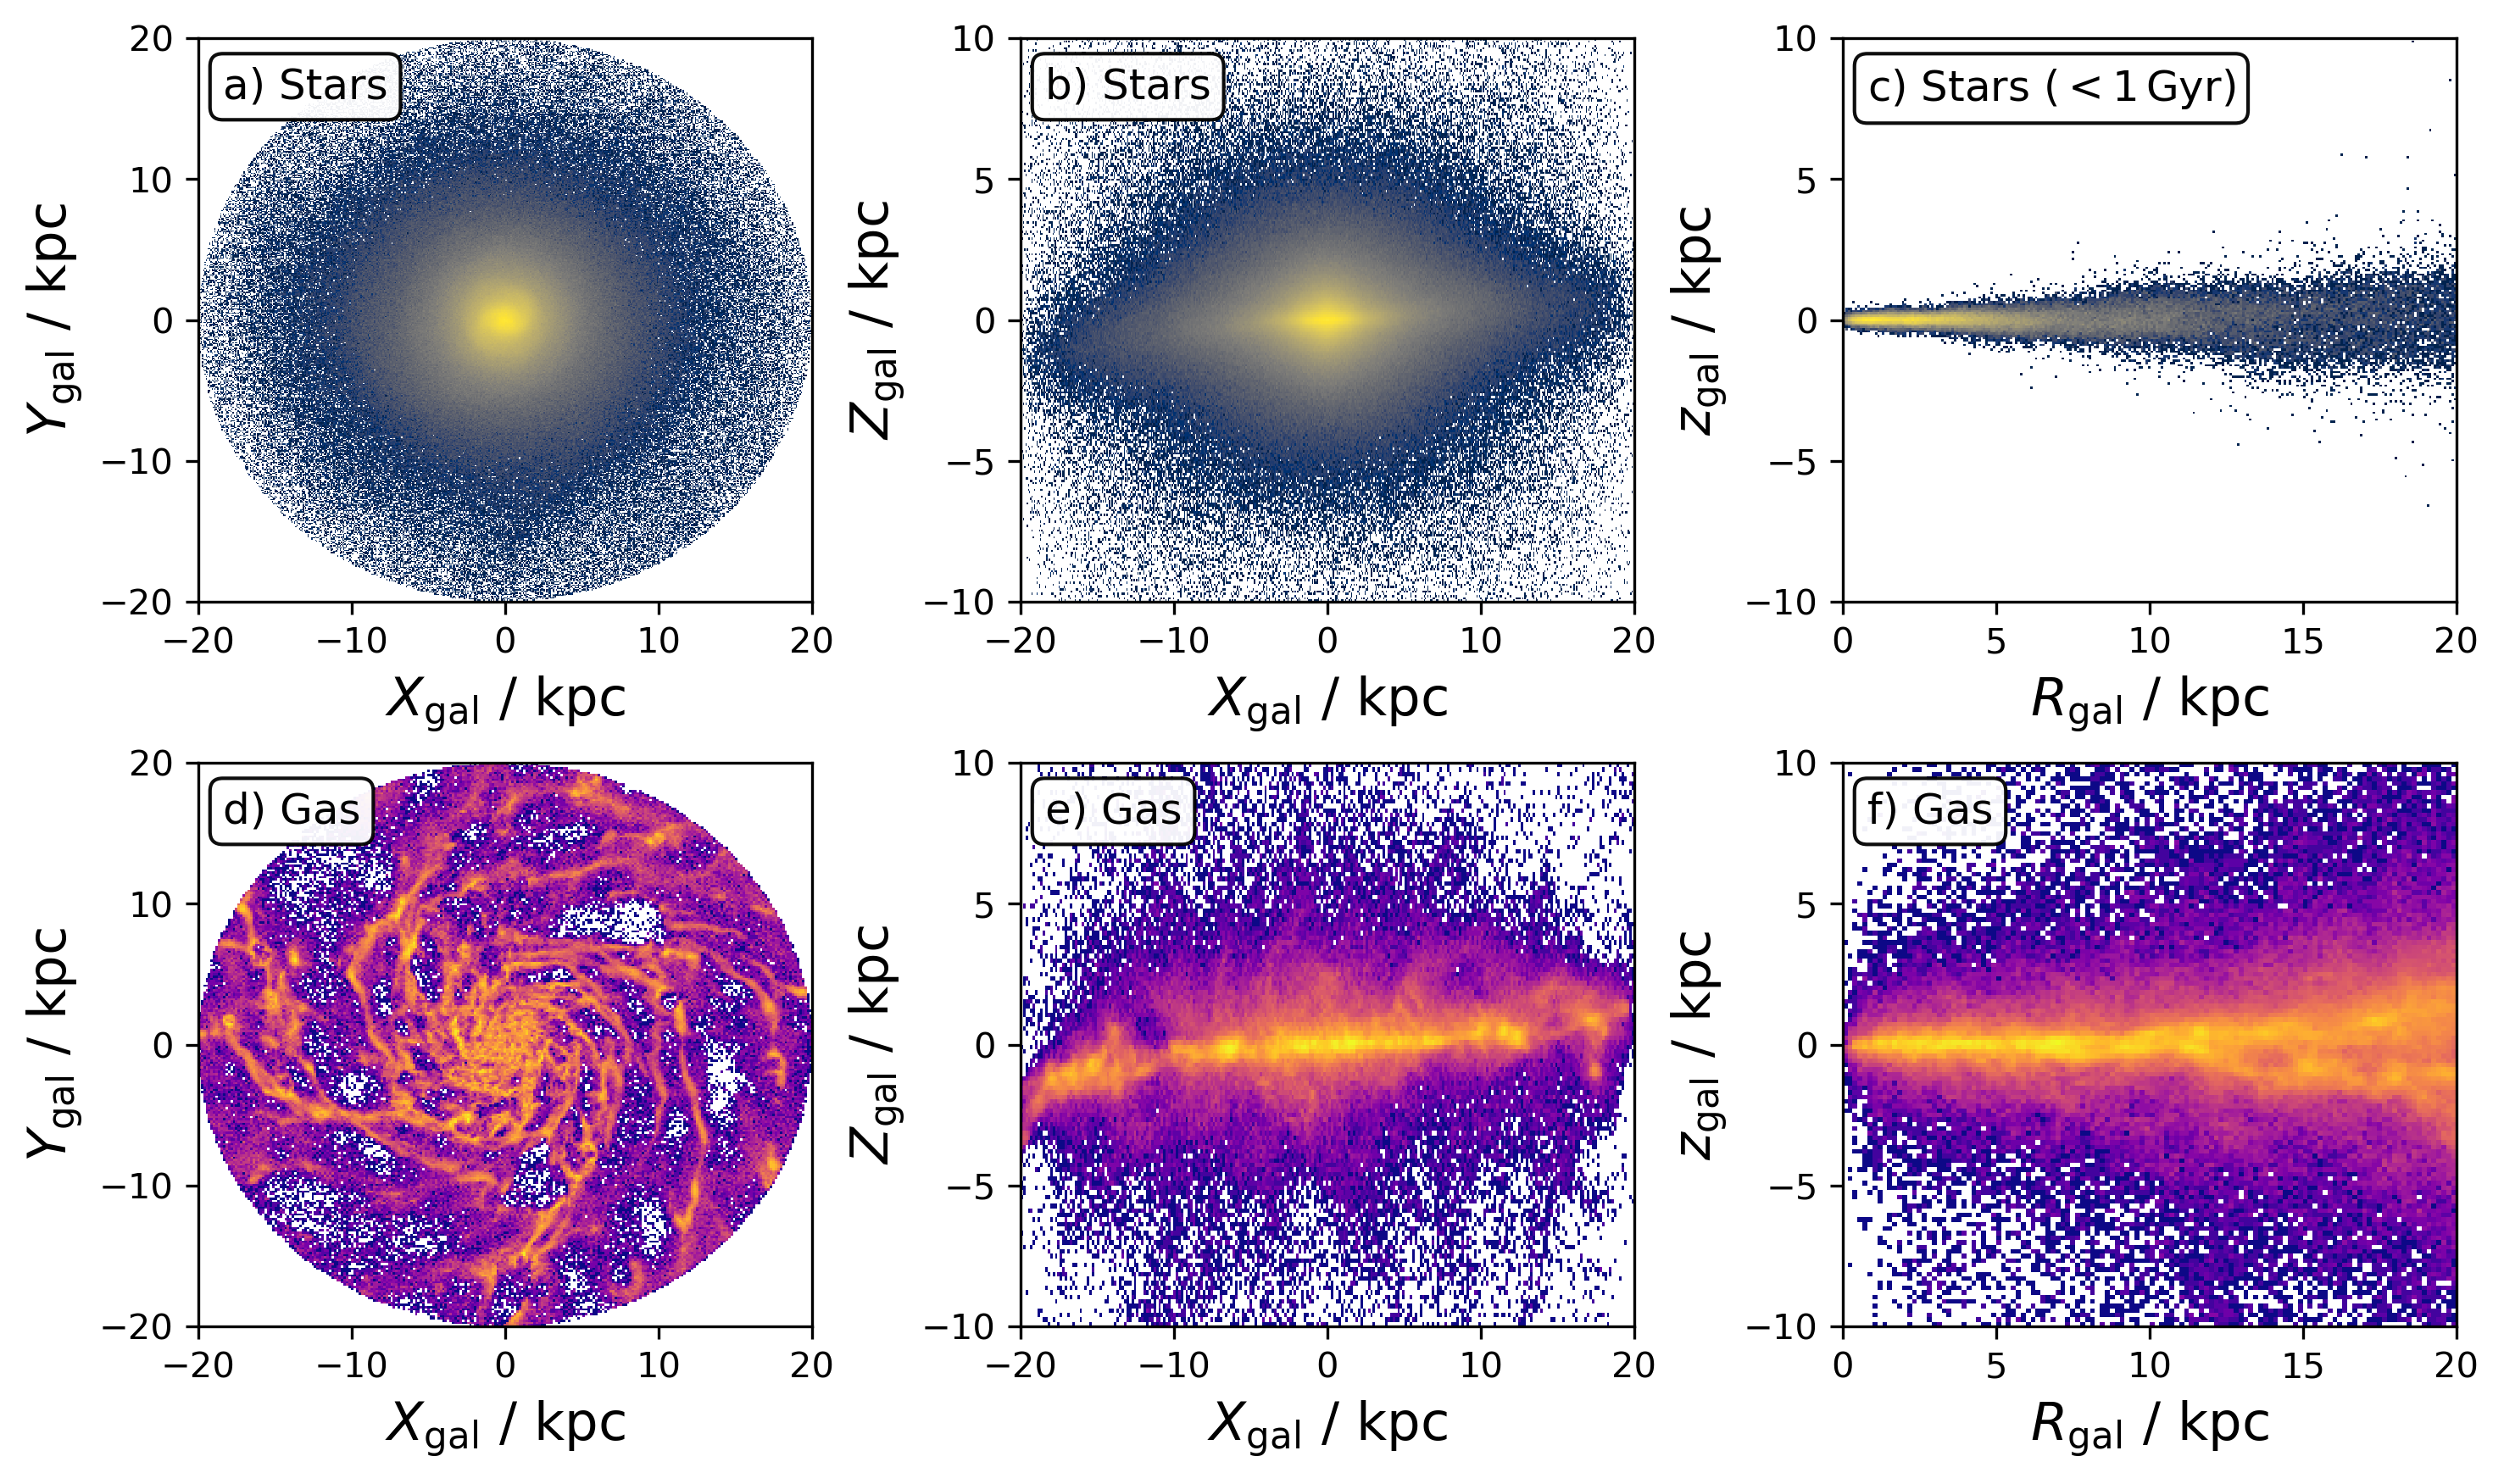
\includegraphics[width=\textwidth]{figures/stars_and_gas_overview.png}
    \caption{Logarithmic spatial density distribution of stars (upper panels) and gass (lower panels) within $R < 20\,\mathrm{kpc}$ of the NIHAO Milky Way analogue \texttt{g8.26e11} galactocentric cartesian and cylindric coordinates. Panel c) shows the influence of selecting only young stars ($<1\,\mathrm{Gyr}$).}
    \label{fig:stars_and_gas_overview}
\end{figure*}

%%%%%%%%%%%%%%%%%%%%%%%%%%%%%%%%%%%%%%%%%%%%%%%%%%

\section{Radial metallicity gradients in NIHAO}
\label{sec:radial_metallicity_gradients}


\subsection{Linearity of the gradient}
\label{sec:linear_radial_metallicity_gradients}

\subsection{Scatter in the gradient}
\label{sec:scatter_radial_metallicity_gradients}

\subsection{Coherence of the gradient with position}

\begin{figure*}
    \centering
    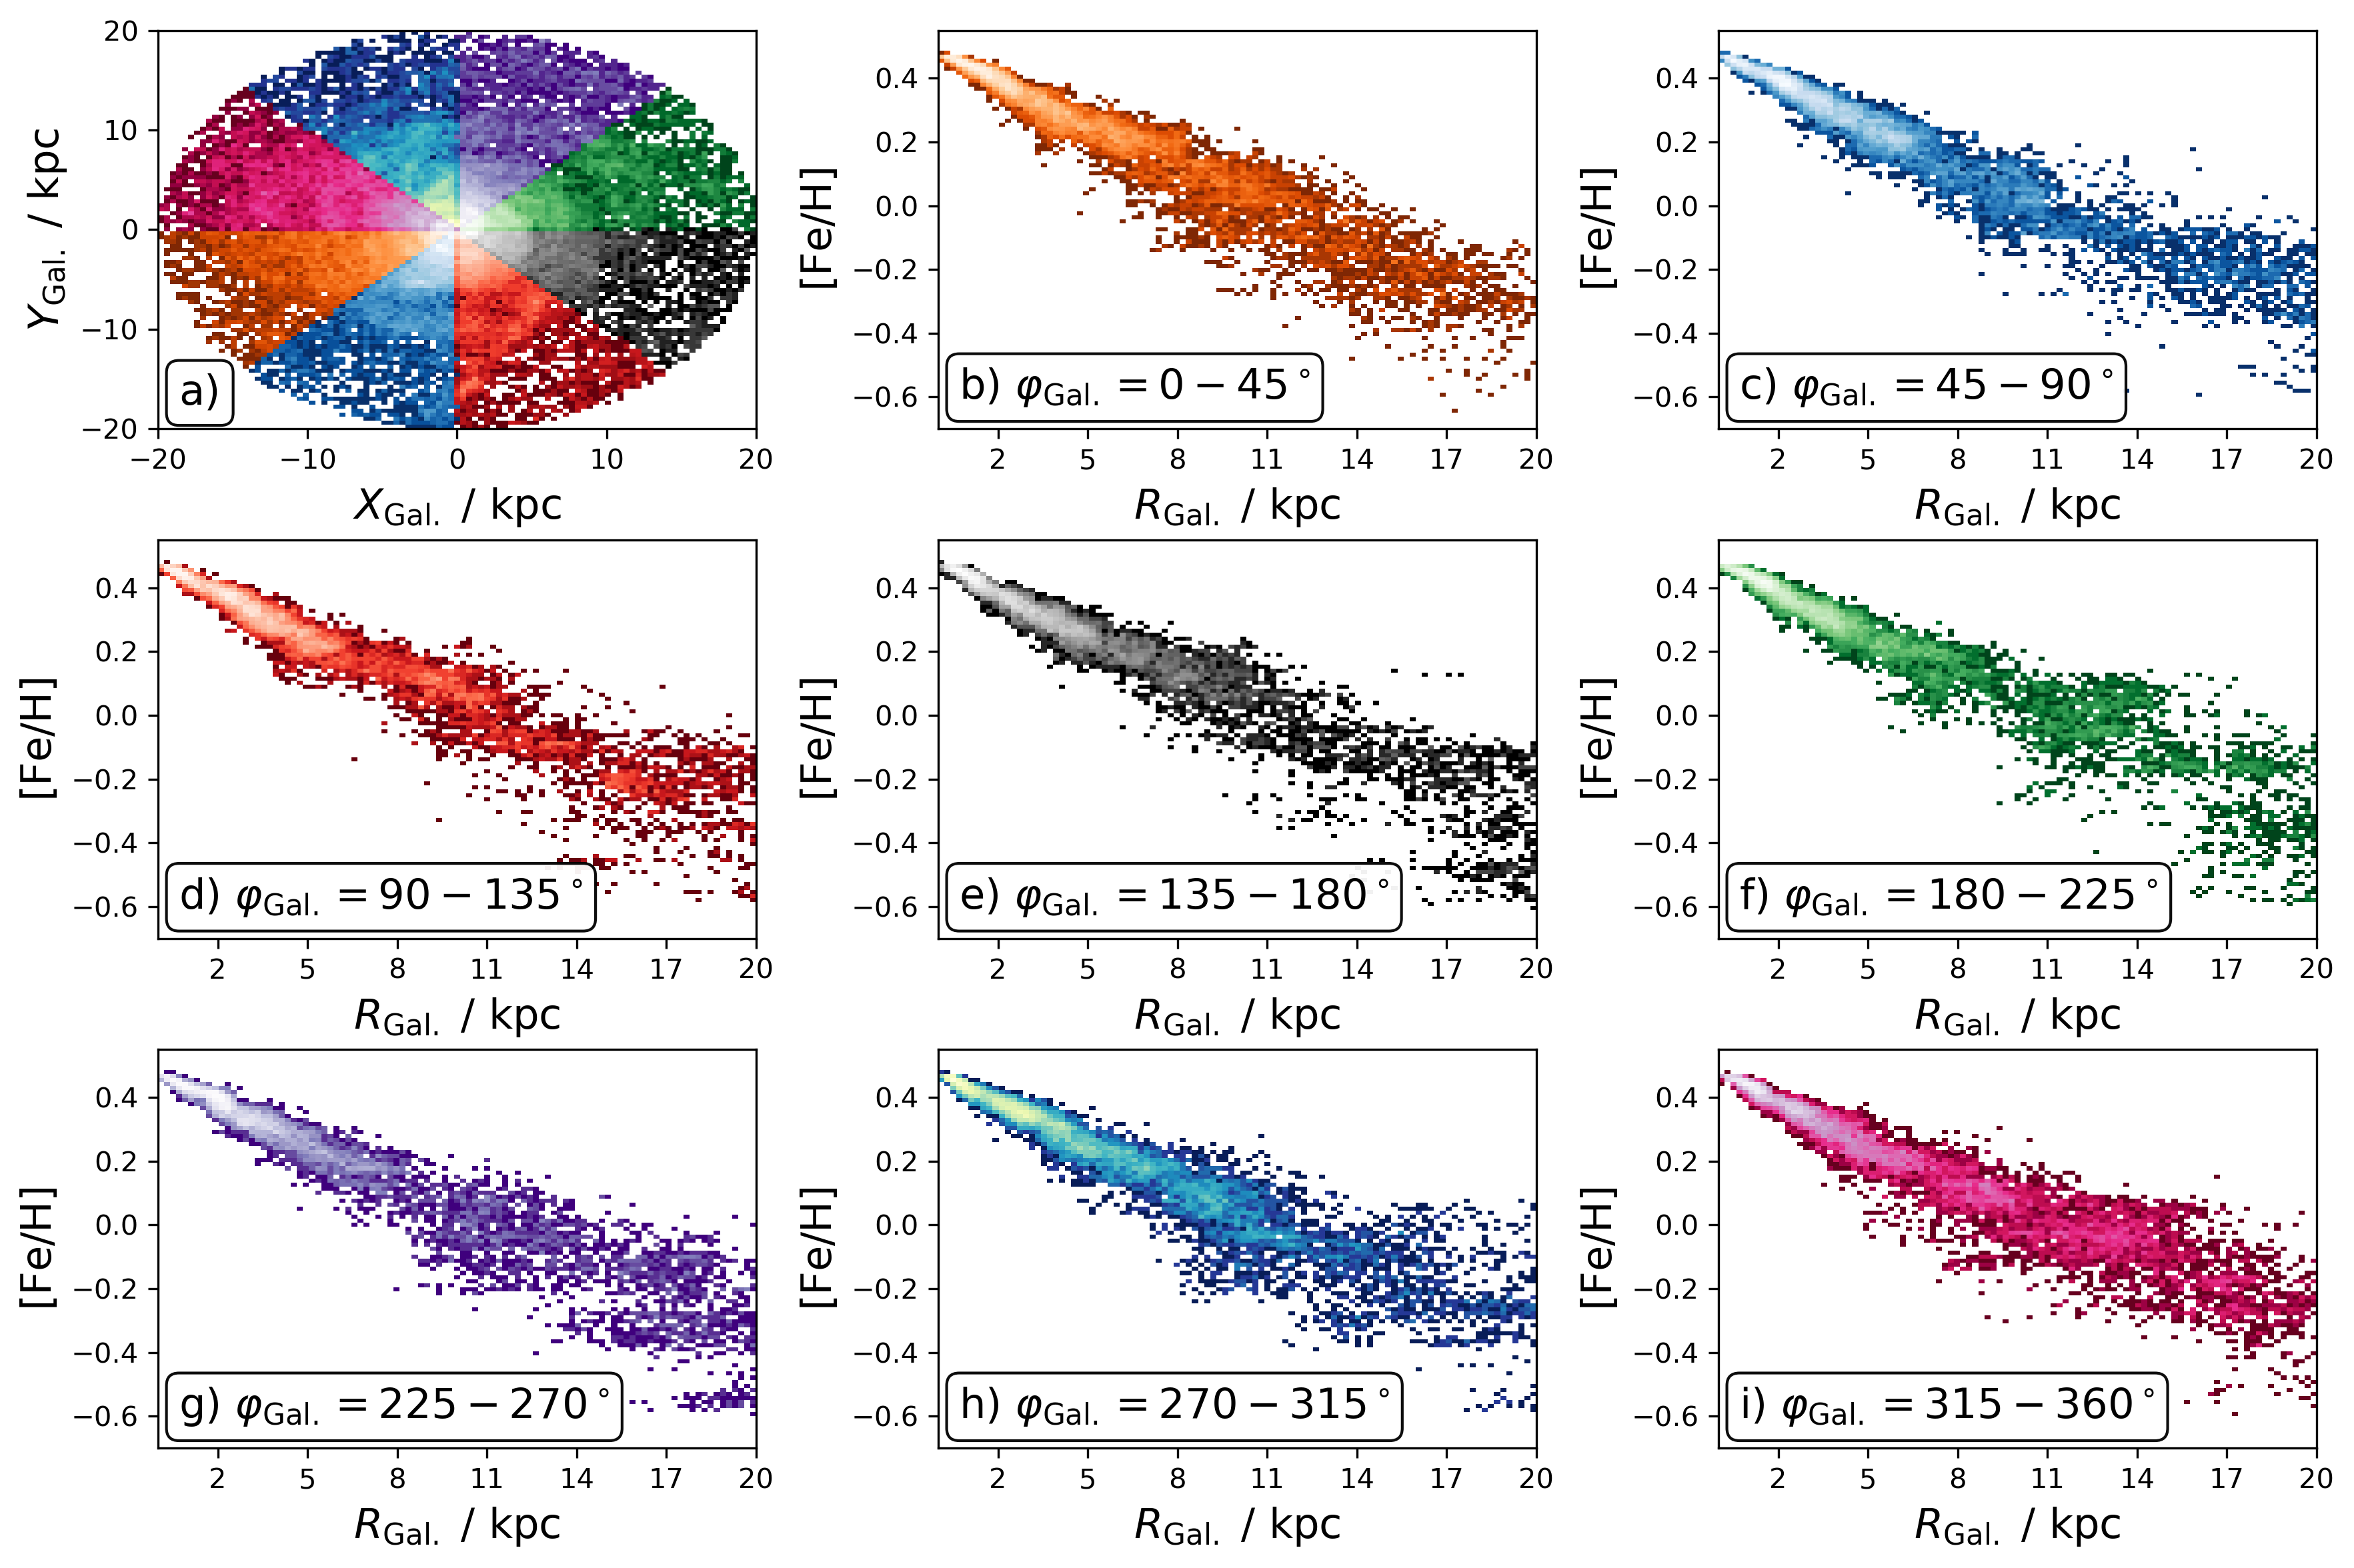
\includegraphics[width=\textwidth]{figures/radial_metallicity_gradients_mw_in_angles.png}
    \caption{Density variation of the radial metallicity gradient $R-\mathrm{[Fe/H]}$ across 8 different sectors. A rotating lighthouse-like GIF animation of the median age and median density of the $R-\mathrm{[Fe/H]}$-relation is freely available on the \href{https://github.com/svenbuder/nihao_radial_metallicity_gradients/blob/main/figures/xyz_rfeh.gif}{github repository}.}
    \label{fig:radial_metallicity_gradients_mw_in_angles}
\end{figure*}

\begin{figure*}
    \centering
    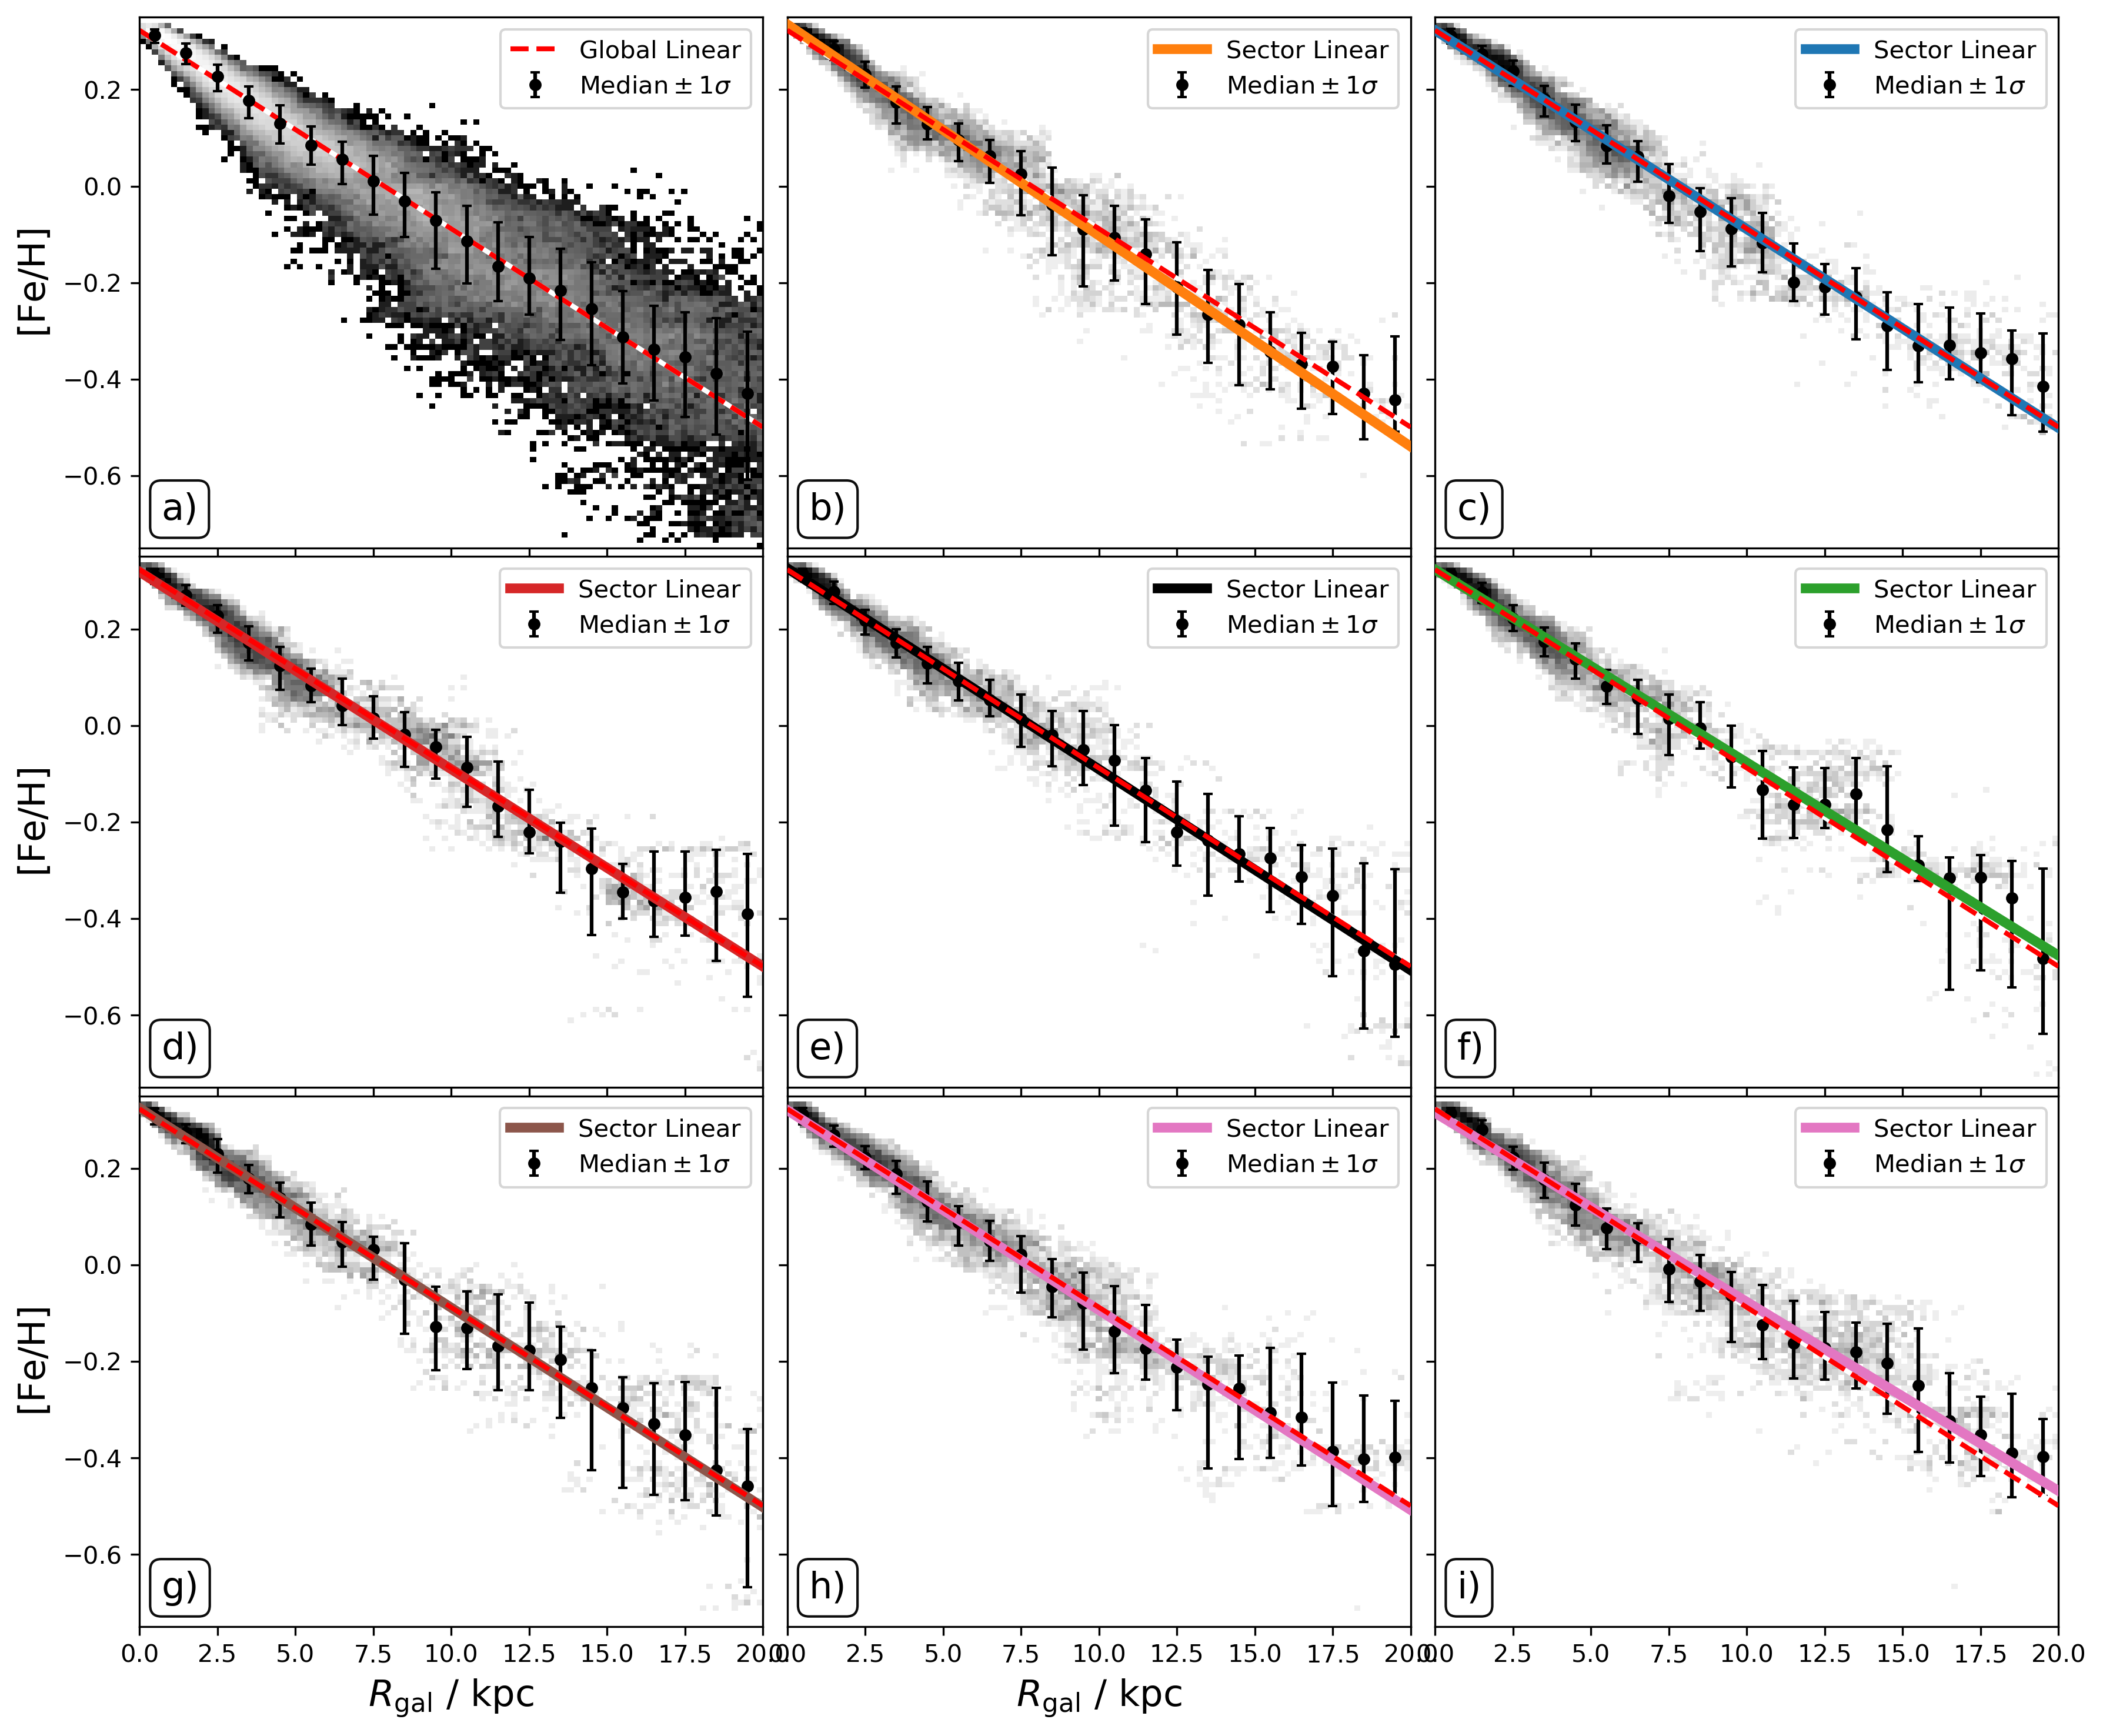
\includegraphics[width=\textwidth]{figures/linear_radial_metallicity_gradients_mw_in_angles.png}
    \caption{Density variation of the radial metallicity gradient $R-\mathrm{[Fe/H]}$ across full stellar disk and 8 different sectors (same panel order as for Fig.~\ref{fig:radial_metallicity_gradients_mw_in_angles}). Linear radial metallicity gradients have been fit globally (red dashed line) and for each sector with colors following the same color code as in Fig.~\ref{fig:radial_metallicity_gradients_mw_in_angles}}.
    \label{fig:linear_radial_metallicity_gradients_mw_in_angles}
\end{figure*}

\subsection{Coherence of the gradient with age}

\SB{Do the same as Fig.~\ref{fig:radial_metallicity_gradients_mw_in_angles}, but with bins colored by median age.}

\SB{Global $R-\mathrm{[Fe/H]}$, then local for the 8 sectors of Fig.~\ref{fig:radial_metallicity_gradients_mw_in_angles}, plot both in 2x4 subpanels, and color-code the density plots by median deviation from this line with a seismic map.}



Fig.~\ref{fig:linear_radial_metallicity_gradients_mw_in_angles}f shows impressively, that if you look at a rather narrow range of $R_\mathrm{gal}$, such as $7 < R_\mathrm{gal} < 13\,\mathrm{kpc}$, the radial metallicity gradient could actually look like it is damping towards larger radii. \SB{Is this possibly what is happening in local studies of our galaxy, where many researchers are actually fitting 2 linear gradients with a break radius?}

\SB{Actually one can see this effect even better in Fig.~\ref{fig:radial_metallicity_gradients_mw_in_angles}b,d,e,f,h and i!}

%%%%%%%%%%%%%%%%%%%%%%%%%%%%%%%%%%%%%%%%%%%%%%%%%%
\section{Discussion} \label{sec:discussion}

Comparison to \citet[][see their Fig. 10]{Minchev2014b}: They see significant decrease of stars towards larger radii (note to myself: their bins are not scatter, but number density in Fig. 10). How does this compare to our number densities?

\subsection{Linearity of the gradient} \label{sec:discussion_linearity}

To what extent is the radial metallicity gradient of young stars linear? Alternatively, would it be better described by two linear relations, with a break radius at corotation radius \citep[][and references therein]{Bresolin2012} or further out \citep{Donor2020} or a more sophisticated function \citep[see e.g.][]{Chiappini2001, Kubryk2015}? Investigating the gradient's form helps in understanding the galactic processes influencing metallicity at different radii \citep{Minchev2014b}.

\SB{Put some of these results into context of the Milky Way in Fig.~\ref{fig:radial_metallicity_gradients_mw_vs_nihao}.}

\begin{figure*}
    \centering
    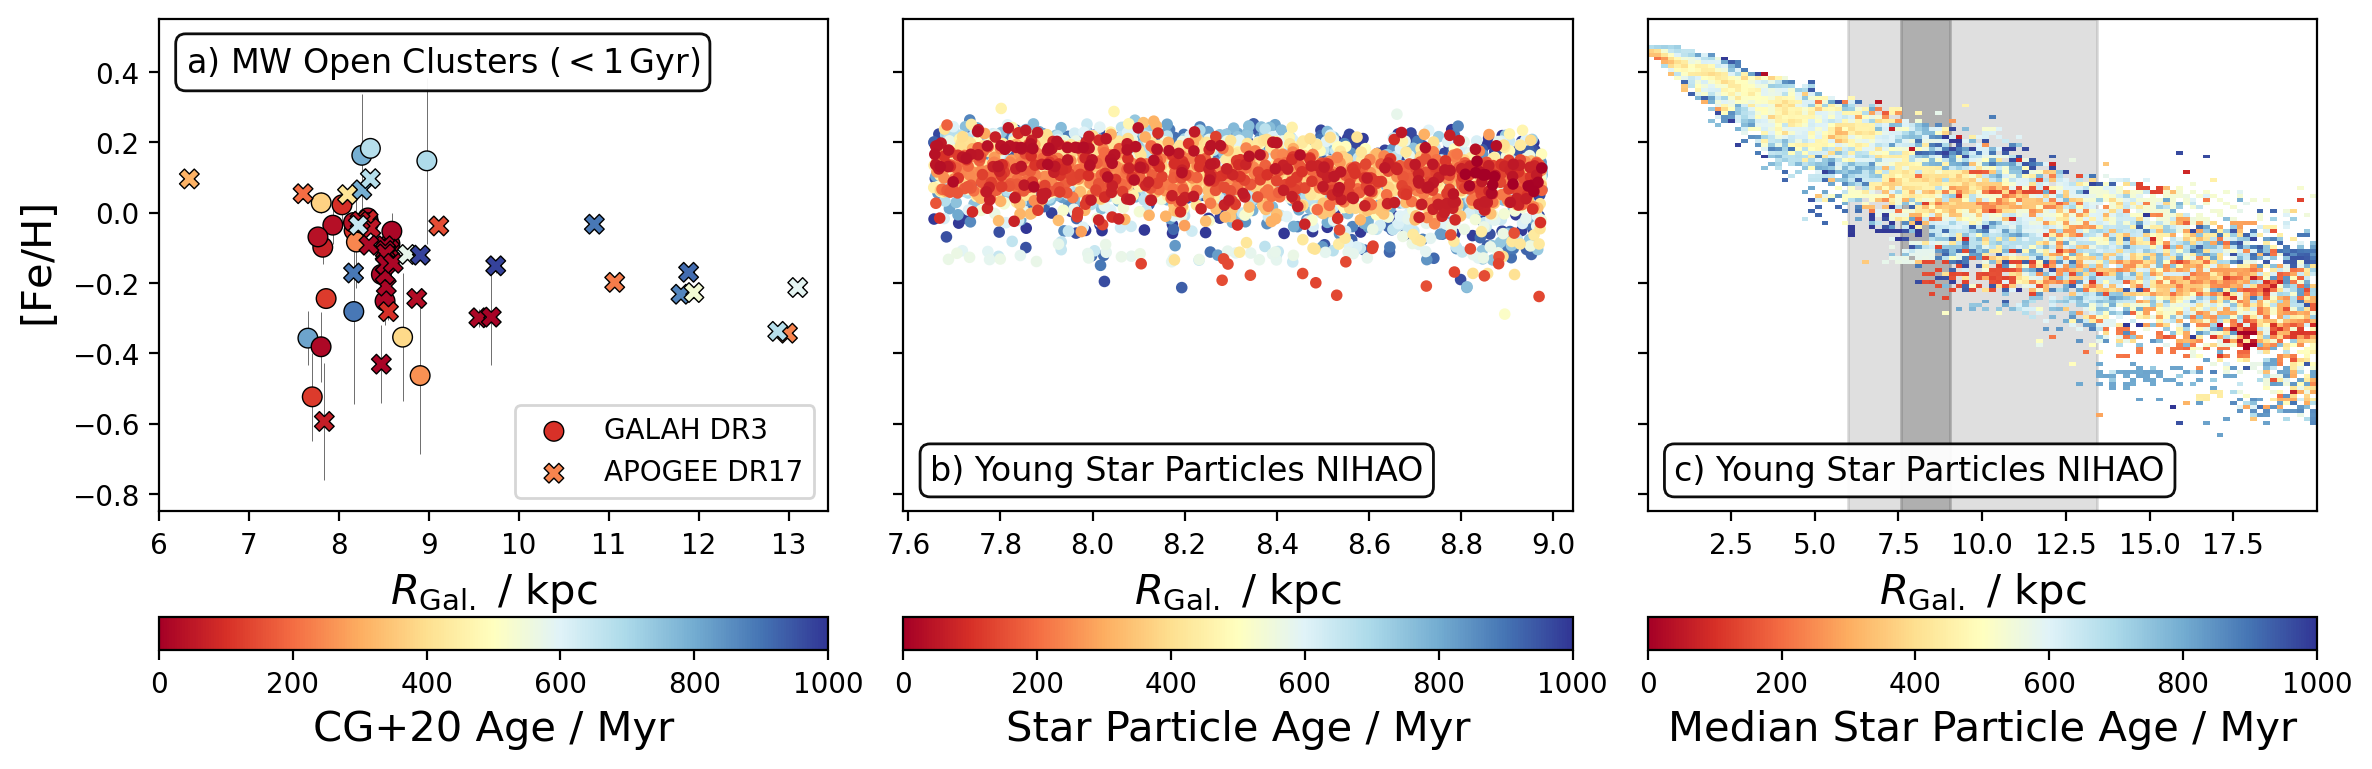
\includegraphics[width=\textwidth]{figures/radial_metallicity_gradients_mw_vs_nihao.png}
    \caption{Caption}
    \label{fig:radial_metallicity_gradients_mw_vs_nihao}
\end{figure*}

\subsection{Scatter in the gradient} \label{sec:discussion_scatter}

How much scatter in the radial metallicity gradient of young stars is expected based on simulations? Quantifying the scatter can provide insights into the effects of transient events like mergers, star formation bursts, and gas accretion.

\SB{Put some of these results into context of the Milky Way in Fig.~\ref{fig:overdensities_mw_vs_nihao}, e.g. \citet{Poggio2021} and \citet{Hackshaw2024}.}

\begin{figure*}
    \centering
    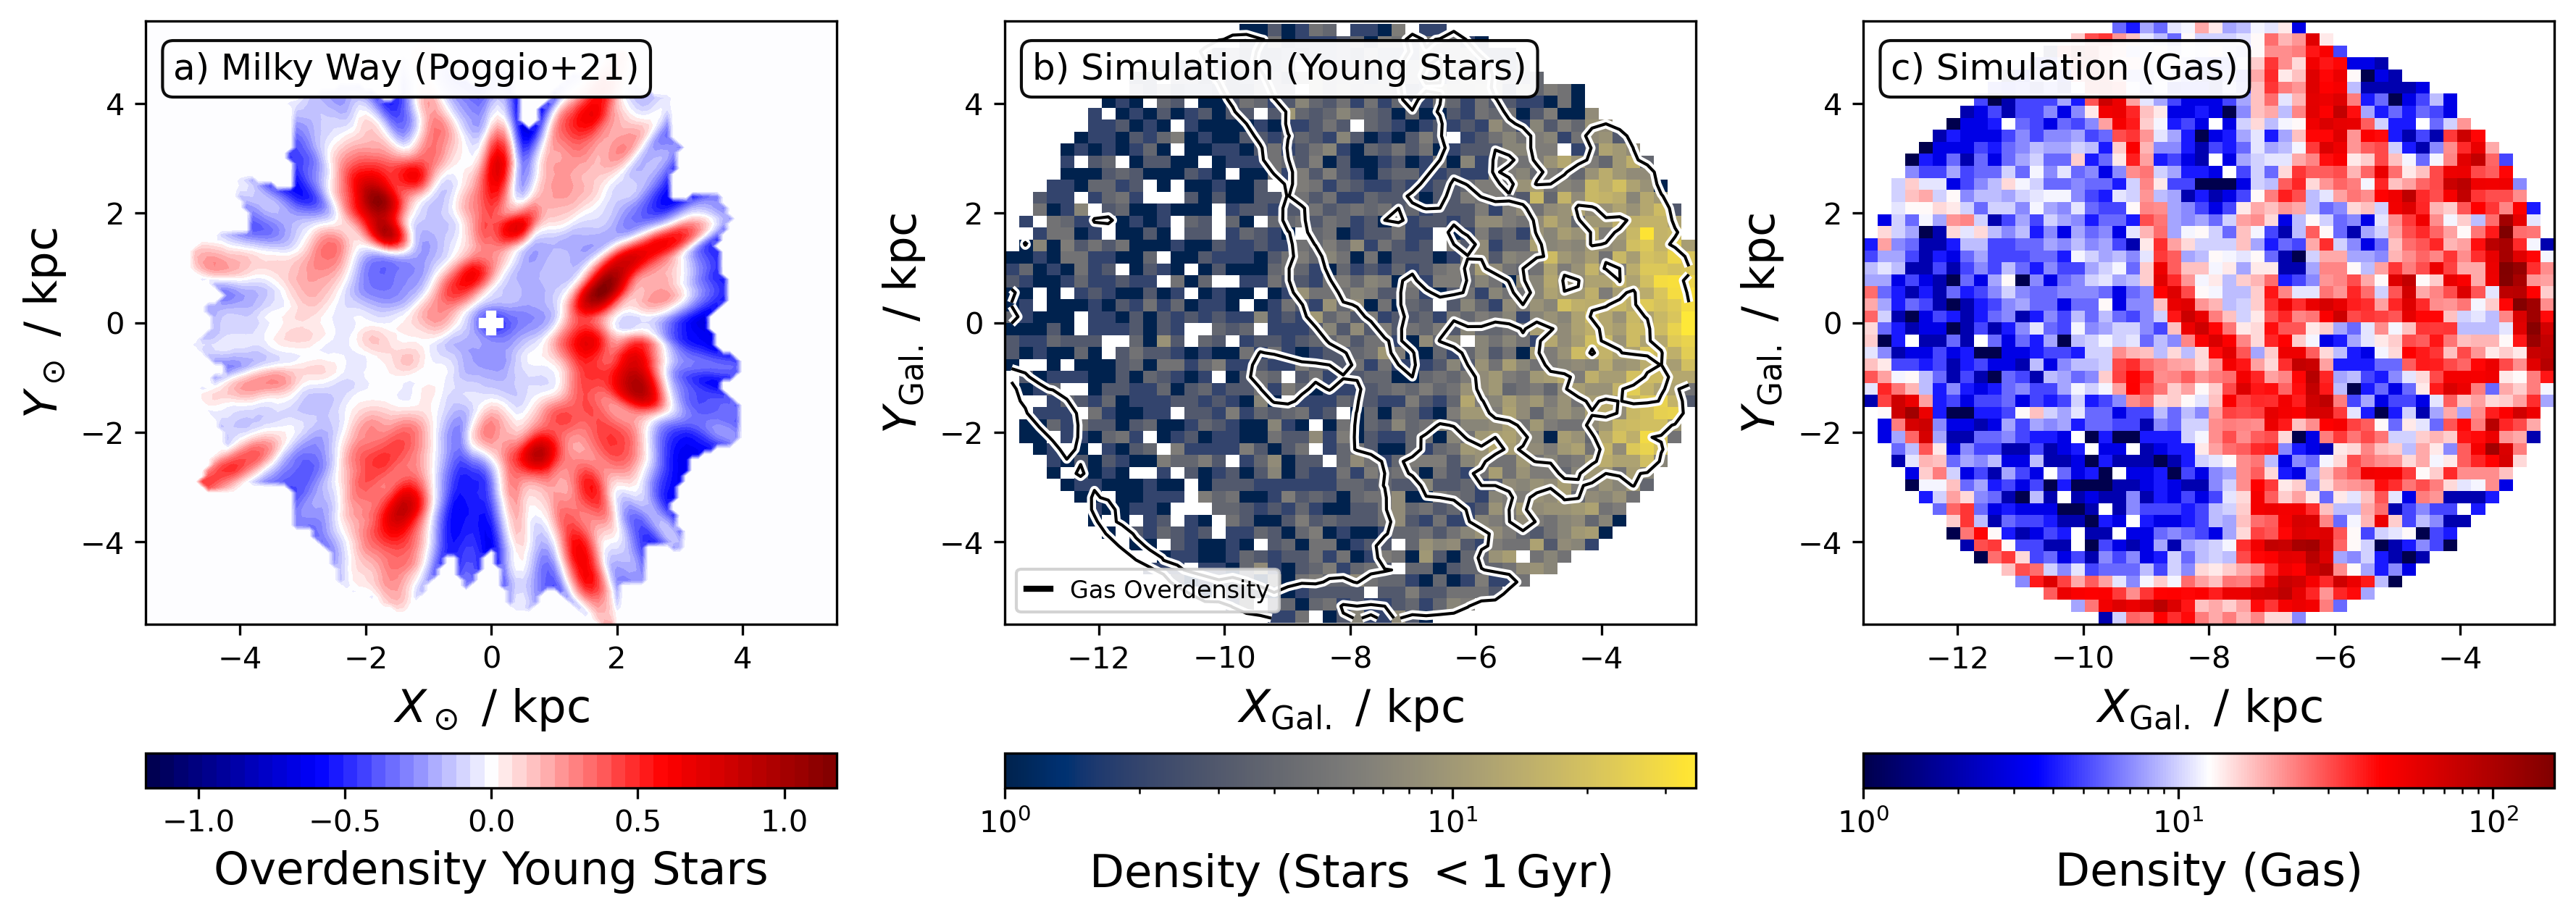
\includegraphics[width=\textwidth]{figures/overdensities_mw_vs_nihao.png}
    \caption{Caption}
    \label{fig:overdensities_mw_vs_nihao}
\end{figure*}

\subsection{Coherence of the gradient with position} \label{sec:discussion_coherence_position}

How significant is the change in the radial metallicity of young stars gradient as a function of position, both in terms of radial coverage and azimuth? Understanding these variations can reveal the underlying processes affecting metallicity distribution, such as spiral arm dynamics and bar-driven mixing \citep[see their Figs. 5-8][]{DiMatteo2013}.

\subsection{Coherence of the gradient with age} \label{sec:discussion_coherence_age}

Until what stellar age can stars be used as reliable tracers of the gas disk in simulations, in terms of both chemical composition and position? This question is pivotal for interpreting observed gradients across different ages \citep[e.g.][]{Willett2023} and comparing them with model predictions, particularly concerning the migration and heating of stellar populations \citep{Binney2008, Frankel2018}.


%%%%%%%%%%%%%%%%%%%%%%%%%%%%%%%%%%%%%%%%%%%%%%%%%%
%%%%%%%%%%%%%%%%%%%%%%%%%%%%%%%%%%%%%%%%%%%%%%%%%%
\section{Conclusions}
\label{sec:conc}


\section*{Acknowledgements}

We acknowledge the traditional owners of the land on which the AAT and ANU stand, the Gamilaraay, the Ngunnawal and Ngambri people. We pay our respects to elders past, present, and emerging and are proud to continue their tradition of surveying the night sky in the Southern hemisphere.

This work was supported by the Australian Research Council Centre of Excellence for All Sky Astrophysics in 3 Dimensions (ASTRO 3D), through project number CE170100013. SB acknowledges support from the Australian Research Council under grant number DE240100150 which enabled SB to continue researching at the end of a fixed-term position and finalising this study. TB acknowledges funding from the Carl Zeiss Stiftung and support from the European Research Council under ERC-CoG grant CRAGSMAN-646955. We gratefully acknowledge the Gauss Centre for Supercomputing e.V. (\url{www.gaus s-centre.eu}) for funding this project by providing computing time on the GCS Supercomputer SuperMUC at Leibniz Supercomputing Centre (\url{www.lrz.de}). Simulations were partially computed with High Performance Computing resources at New York University, Abu Dhabi.

\section*{Facilities}

\textbf{AAT with 2df-HERMES at Siding Spring Observatory:} The GALAH Survey is based data acquired through the Australian Astronomical Observatory, under programs: A/2013B/13 (The GALAH pilot survey); A/2014A/25, A/2015A/19, A2017A/18 (The GALAH survey phase 1), A2018 A/18 (Open clusters with HERMES), A2019A/1 (Hierarchical star formation in Ori OB1), A2019A/15 (The GALAH survey phase 2), A/2015B/19, A/2016A/22, A/2016B/10, A/2017B/16, A/2018B/15 (The HERMES-TESS program), and A/2015A/3, A/2015B/1, A/2015B/19, A/2016A/22, A/2016B/12, A/2017A/14, (The HERMES K2-follow-up program). This paper includes data that has been provided by AAO Data Central (\url{datacentral.aao.gov.au}).

\textbf{\Gaia: } This work has made use of data from the European Space Agency (ESA) mission \Gaia (\url{http://www.cosmos.esa.int/gaia}), processed by the \Gaia Data Processing and Analysis Consortium (DPAC, \url{http://www.cosmos.esa.int/web/gaia/dpac/consortium}). Funding for the DPAC has been provided by national institutions, in particular the institutions participating in the \Gaia Multilateral Agreement. 

\textbf{Other facilities:} This publication makes use of data products from the Two Micron All Sky Survey \citep{Skrutskie2006} and the CDS VizieR catalogue access tool \citep{Vizier2000}.

\section*{Software}

The research for this publication was coded in \textsc{python} (version 3.7.4) and included its packages
\textsc{astropy} \citep[v. 3.2.2;][]{Robitaille2013,PriceWhelan2018},
\textsc{IPython} \citep[v. 7.8.0;][]{ipython},
\textsc{matplotlib} \citep[v. 3.1.3;][]{matplotlib},
\textsc{NumPy} \citep[v. 1.17.2;][]{numpy},
\textsc{pynbody} \citep[v. 1.1.0;][]{pynbody},
\textsc{scipy} \citep[version 1.3.1;][]{scipy},
We further made use of \textsc{topcat} \citep[version 4.7;][]{Taylor2005};

%%%%%%%%%%%%%%%%%%%%%%%%%%%%%%%%%%%%%%%%%%%%%%%%%
\section*{Data Availability}

All code and data to reproduce the analysis and figures can be accessed via \url{https://github.com/svenbuder/age_abundance_nihao_vs_galah}.

% The repository also includes the chemical and kinematic data of the simulated Milky Way analogue \texttt{g8.26e11} for last snapshot of the simulation for the observable footprint that were used for this study as well as the cleaned catalogue of GALAH DR3. All GALAH DR3 data is also published by \citet{Buder2021} and can be accessed publicly via \url{https://docs.datacentral.org.au/galah/dr3/overview/}. The full simulation data of \texttt{g8.26e11} can be obtained upon reasonable request from the authors. Currently the only limitation in making all data public is limited cloud space to host the data. We encourage interested readers to get in contact with the authors for full data access. Redshift zero snapshots from the original NIHAO-UHD simulations can be found here: \url{https://tobias-buck.de/\#sim_data}.

% If you are using either of these data to follow up on this research, remember to give appropriate credit to the researchers who created and curated either data set, that is, at least to \citet{Buder2021, Buder2022} and \citet{Buck2020b, Buck2021}.

%%%%%%%%%%%%%%%%%%%% REFERENCES %%%%%%%%%%%%%%%%%%

% The best way to enter references is to use BibTeX:
\bibliographystyle{mnras}
\bibliography{bib} % if your bibtex file is called example.bib

%%%%%%%%%%%%%%%%%%%%%%%%%%%%%%%%%%%%%%%%%%%%%%%%%%
%%%%%%%%%%%%%%%%% APPENDICES %%%%%%%%%%%%%%%%%%%%%

% \newpage
% \appendix


%%%%%%%%%%%%%%%%%%%%%%%%%%%%%%%%%%%%%%%%%%%%%%%%%%
% Don't change these lines
\bsp	% typesetting comment
\label{lastpage}
\end{document}